\documentclass[10pt]{article}
\usepackage[latin1]{inputenc}
\usepackage[french]{babel}
\usepackage[rigidchapters]{titlesec}
\usepackage{comment,fullpage}
\usepackage{hyperref}
\usepackage{comment,times,fancyvrb,amsmath,amsthm,amssymb,latexsym,xspace}
\usepackage{graphicx}

\graphicspath{./Fig}

% Palatino for rm and math | Helvetica for ss | Courier for tt
\usepackage{mathpazo} % math & rm
\linespread{1.05}        % Palatino needs more leading (space between lines)
\usepackage[scaled]{helvet} % ss
\usepackage{courier} % tt
\normalfont

\usepackage[T1]{fontenc}
\usepackage{listings}
\usepackage{color}
\usepackage{lastpage}
\usepackage{verbatim}
\usepackage{enumitem}
 
\newenvironment{correction}{~\linebreak%
\color{red}
%\textbf{\rule{4cm}{0.05cm}\linebreak
Correction\,:\linebreak
}%}{\hfill~\linebreak\rule{4cm}{0.05cm}}

%\includecomment{comment}
%\excludecomment{comment}
\excludecomment{correction}

\setenumerate[0]{font=\itshape, label*=\thesection.\arabic*}


\newcommand{\entete}[2]{\begin{center}
{\Large Syst\`emes de gestion de bases de donn\'ees \\NFP 107#1, CNAM Paris\\
#2\\
Examen de 2 heures 30\\
{\large (Tous documents autoris\'es)}}
\end{center}

\noindent
\textbf{Consignes\,:}
\begin{itemize}
  \item Pensez \`a reporter votre num\'ero d'anonymat sur toutes les feuilles.
  \item  Merci
de soigner votre \'ecriture et de ne pas r\'ediger au crayon papier sur votre copie. 
\item Eteignez vos t\'el\'ephones portables. Ceux-ci ne sont pas
autoris\'es, m\^eme pas pour servir d'horloge.
\end{itemize}
Ce sujet comporte \pageref{LastPage} pages d'\'enonc\'e.}

\begin{document}

\entete{HTT}{Septembre 2015}

\section{Alg�bre relationnelle et SQL (10 points)}
Voici une partie de la base de donn�es d'un site g�rant la r�servation de billets pour des
concerts~:
\begin{verbatim}
FORMATION(nom, ann�eFormation, nombreMembres, pays)
SALLE(nomSalle, typeSalle, ville, capacit�)
CONCERT(codeConcert, nomFormation, nomSalle, dateConcert, nbBilletsVendus)
BILLET(idBillet, codeConcert, prix)
\end{verbatim}
Pour une formation sont stock�s son nom, l'ann�e o� l'artiste/le groupe a d�but�, le nombre de membres composant le groupe (1 pour un artiste en solo) et son pays d'origine.
Pour la salle nous connaissons son nom, son type (stade, ar�ne, petite salle, grande salle, etc), sa ville et son nombre de places. Les concerts sont identifi�s par un code, donn�s par une formation, se d�roulent dans une salle, ont lieu � une date et ont un nombre de billets vendus. Les billets ont un identifiant, un code concert et un prix.

\begin{enumerate}

\item Pour la table CONCERT, identifiez la cl� primaire et les cl�s �trang�res (0,5 points)\\
\begin{correction}
Cl� primaire: codeConcert\\
Cl�s �trang�res: nomSalle$\rightarrow$SALLE.nomSalle, nomFormation$\rightarrow$FORMATION.nom
\end{correction}

\item Donnez la commande SQL pour cr�er la table CONCERT. (0.5 point)\\
\begin{correction}
\begin{verbatim}
CREATE TABLE CONCERT(
    codeConcert NUMBER(10),
    nomFormation VARCHAR(50),
    nomSalle VARCHAR(50)
    dateConcert DATE,
    nbBilletsVendus NUMBER(10),
    CONSTRAINT pk_concert PRIMARY_KEY (codeConcert),
    CONSTRAINT fk_concert FOREIGN_KEY (nomSalle) REFERENCES SALLE(nomSalle),
    CONSTRAINT fk_concert FOREIGN_KEY (nomFormation) REFERENCES FORMATION(nom))
\end{verbatim}
\end{correction}
% on peut am�liorer les types et ajouter des contraintes mais on ne leur en pas beaucoup parl�, mieux vaut en rester l�

\item (Alg�bre et SQL) Donnez toutes les salles de Paris qui ont plus de 2000 places. (1 point)\\
\begin{correction}
Alg�bre: $\pi_{nomSalle}(\sigma_{ville = Paris \wedge capacite \geq 2000}(SALLE)$
\begin{verbatim}
SELECT nomSalle
FROM SALLE
WHERE ville = 'Paris' AND capacit� > 2000;
\end{verbatim}
\end{correction}

\item (Alg�bre et SQL) Donnez les pays des formations dont au moins un billet co�te plus de 200 euros. (2 points)\\
\begin{correction}
Alg�bre: $\pi_{pays}((BILLET \Join CONCERT)\Join_{nomFormation=nom} FORMATION)$
\begin{verbatim}
SELECT pays
FROM FORMATION f, CONCERT c, BILLET b
WHERE b.codeConcert = c.codeConcert AND C.nomFormation = f.nom AND prix > 200;
\end{verbatim}
\end{correction}

\item (SQL seulement) Donnez le nom des formations qui ont fait la recette (rentr�e d'agent) la plus grande tous concerts confondus en septembre 2015 au Stade de France. (2 points)\\
\begin{correction}
\begin{verbatim}
SELECT nomFormation 
FROM SALLE s, CONCERT c, BILLET b
WHERE s.nomSalle = c.nomSalle AND c.codeConcert = b.codeConcert
      AND dateConcert BETWEEN '01/09/2015' AND '30/09/2015';
GROUP BY nomFORMATION
HAVING SUM(nbBilletsVendus*prix) = 
             (SELECT MAX(SUM(nbBilletsVendus*prix)) 
              FROM SALLE s, CONCERT c, BILLET b
              WHERE s.nomSalle = c.nomSalle 
                    AND c.codeConcert = b.codeConcert;
                    AND dateConcert BETWEEN '01/09/2015' AND '30/09/2015';
              GROUP BY nomFORMATION)
\end{verbatim}
\end{correction}

\item (Alg�bre et SQL) Donnez le nom des formations qui n'ont jamais donn� un concert dans une salle plus petite de 10000 places. (2 points)\\
\begin{correction}
Alg�bre: $\pi_{nom}(FORMATION) - \rho_{nomFormation\rightarrow nom}(\pi_{nomFormation}(\sigma_{capacit� < 10000}((CONCERT \Join SALLE)))$
\begin{verbatim}
SELECT nom
FROM FORMATION
WHERE nom NOT IN 
       SELECT nomFORMATION
       FROM CONCERT c, SALLE s
       WHERE c.nomSalle = s.nomSalle AND capacit� < 10000;
\end{verbatim}
\end{correction}

\item (Alg�bre seulement) Donnez le nom des formations qui ont jou� dans toutes les salles. (Attention~: deux salles situ�es dans des villes diff�rentes peuvent avoir le m�me nom) (1 point)\\
\begin{correction}
$A = \pi_{nomFormation, nomSalle, Ville}(CONCERT \Join SALLE)$ \\
$B = \pi_{nomSalle, Ville}(SALLE)$\\
$Resultat = A \div B$
\end{correction}

\item (Alg�bre seulement) Donnez le nom de la formation qui a vendu le plus de billets pour un concert. (1 point)\\

\begin{correction}
$
CONCERT' = \rho_{attribut\rightarrow attribut'}(CONCERT)\\
\pi_{nomFormation}(CONCERT)-\pi_{nomFormation}(CONCERT \Join_{nbBilletsVendus < nbBilletsVendus'} CONCERT')
$
\end{correction}


\end{enumerate}
 
\section{Index (3 points)}

\begin{enumerate}
  \item Cr�er un index en arbre B d'ordre 2 sur le prix des billets. Les valeurs des cl�s sont donn�es en bas. Montrez chaque �tape d'�clatement de l'arbre. (2 points)
\begin{center}
prix : 100, 95, 110, 120, 80, 85, 130, 90, 75, 125, 115, 60, 70, 140, 135, 65, 145
\end{center}


\begin{correction}
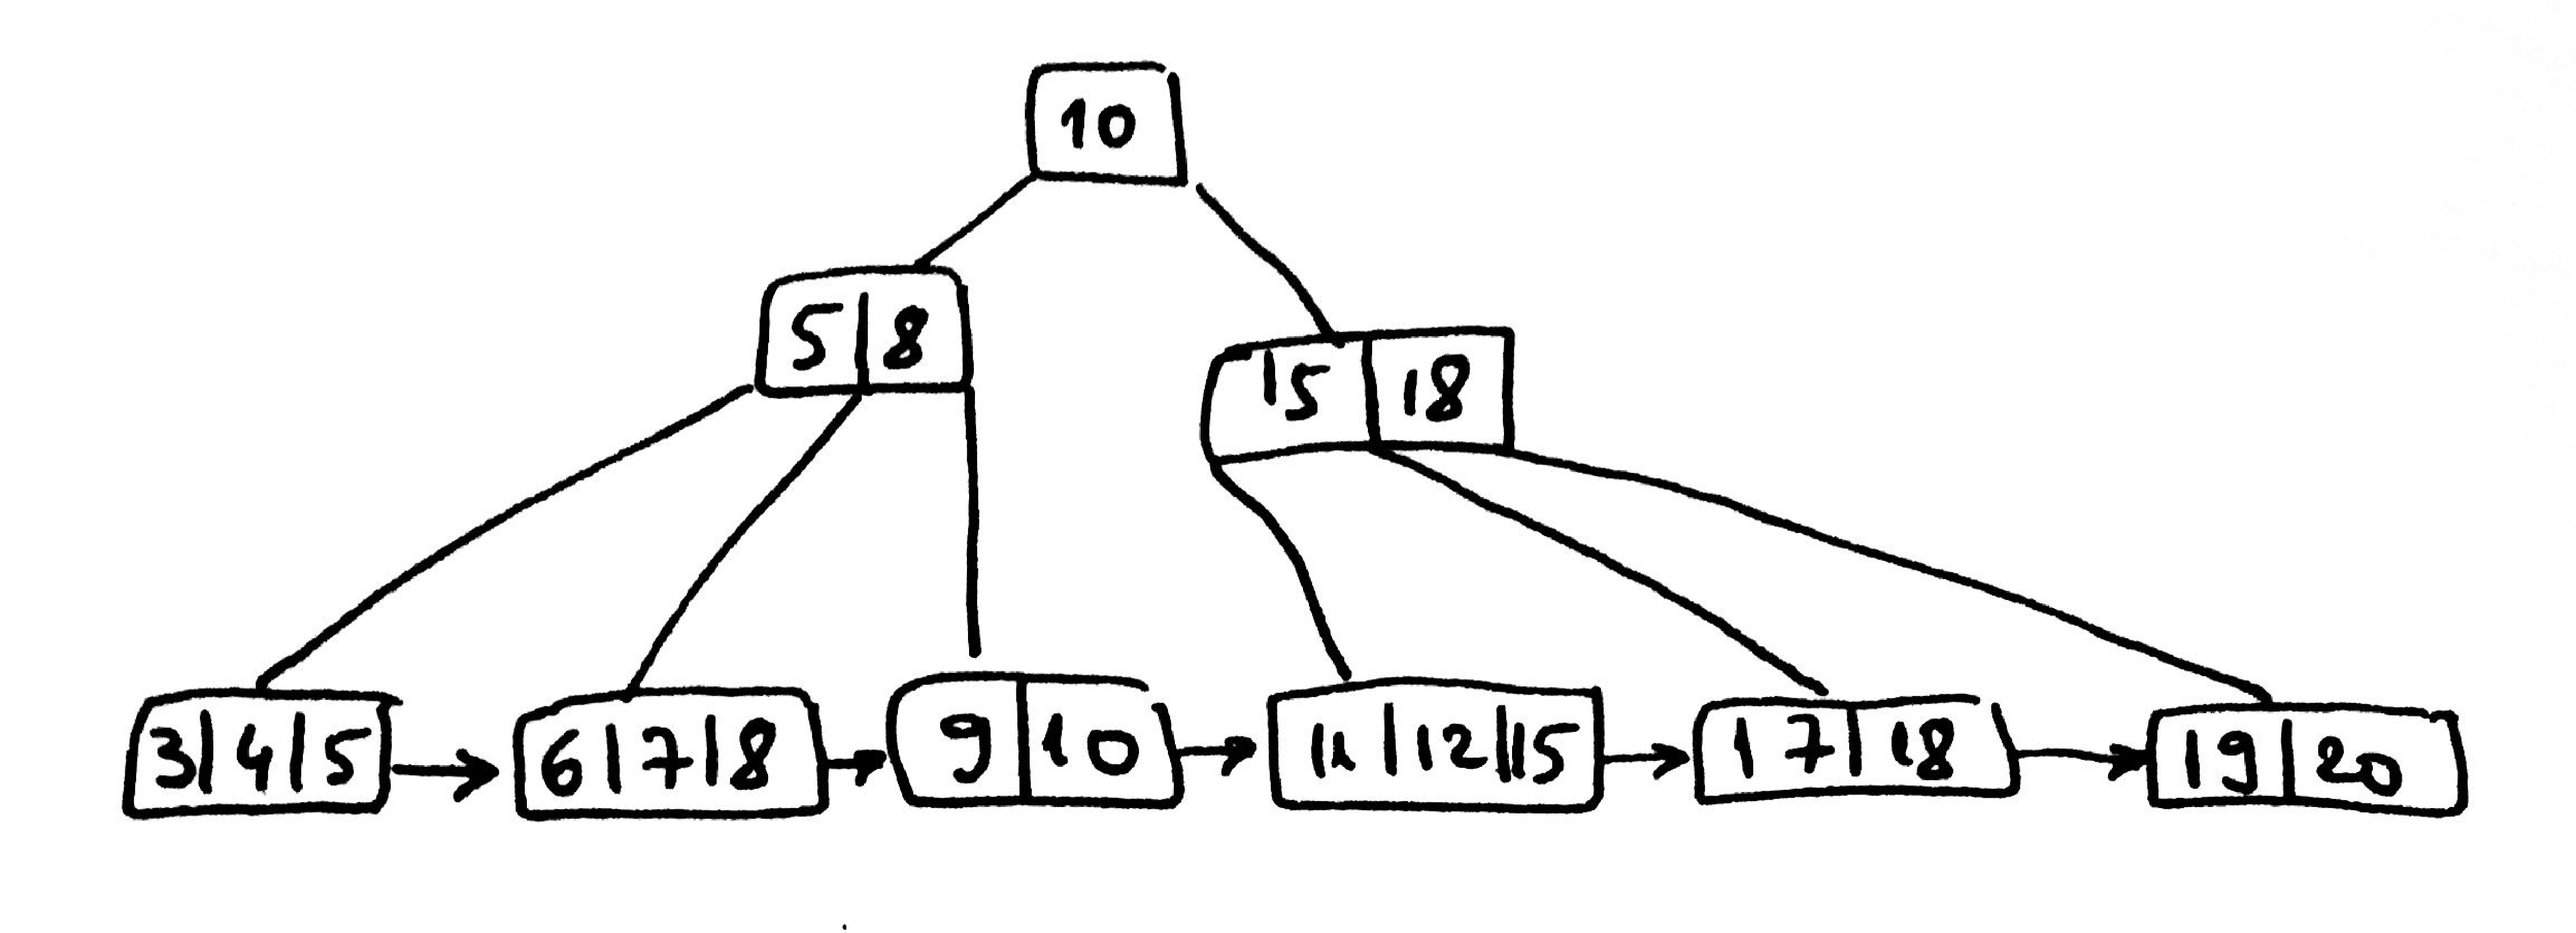
\includegraphics[width=15cm]{Fig/Sujet2.pdf}

\end{correction}

  \item Combien de n\oe{}uds faut-il traverser pour faire une lecture par intervalle des valeurs entre 80 et 130 (dans l'arbre cr�� au point pr�c�dent) ? L'utilisation d'un arbre B+ peut am�liorer cette valeur ? Justifiez. (1 point)

\begin{correction}
On traverse l'arbre de gauche a droite en suivant les fl�ch�s rouges, donc on visite 12 n\oe{}uds (parfois un n\oe{}ud est visit� plusieurs fois). L'arbre B+ peut am�liorer beaucoup cette valeur, car une fois descendu dans les feuilles il suffit de lire � droite dans la liste cha�n�e les valeurs successives.
\end{correction}
\end{enumerate}

\section{Optimisation (4 points)}

Soit la requ�te suivante~:
\begin{verbatim}
SELECT nbBilletsVendus
FROM SALLE s, CONCERT c
WHERE s.nomSalle = c.nomSalle AND s.ville='Paris';
\end{verbatim}

On suppose qu'il y un index sur l'attribut nomSalle dans la table CONCERT.


\begin{enumerate}
  \item Donnez un plan d'ex�cution (arborescente ou EXPLAIN) produit par l'optimiseur pour la requ�te. \textbf{Argumentez}  votre r�ponse. (2 points)

\begin{correction}

L'index CONCERT(nomSalle) permet de faire une recherche sur nomSalle. La cl� � chercher vient donc de l'autre table, SALLE, qui doit �tre parcourue en s�quentiel.

\begin{verbatim}
0 SELECT STATEMENT
1   NESTED LOOPS
2     TABLE ACCESS FULL SALLE
3     TABLE ACCESS BY ROWID CONCERT
5          INDEX RANGE SCAN CONCERT_NOMSALLE_IDX
\end{verbatim}
\end{correction}


\item Comment peut-on acc�l�rer encore la requ�te en ajoutant des index suppl�mentaires~?  Donnez le plan d'ex�cution (arborescente ou EXPLAIN). (2 points)

\begin{correction}
On peut �liminer le parcours s�quentiel de la table SALLE, car la requ�te s'int�resse seulement aux salles situ�es � Paris. Pour cela on ajoute un index sur SALLE(ville) et le plan EXPLAIN devient~:
\begin{verbatim}
0 SELECT STATEMENT
1   NESTED LOOPS
3     TABLE ACCESS BY ROWID SALLE
4          INDEX RANGE SCAN SALLE_VILLE_IDX
5     TABLE ACCESS BY ROWID CONCERT
6          INDEX RANGE SCAN CONCERT_NOMSALLE_IDX
\end{verbatim}
\end{correction}
\end{enumerate}

\section{Concurrence (3 points)}

Soit l'histoire d'ex�cution suivante~:

$H=r_3(z)w_2(x)w_3(z)r_1(x)r_2(y)w_1(x)r_3(y)r_1(x)c_3r_2(z)w_2(x)c_2c_1$


\begin{enumerate}
	\item Donnez la liste des conflits de H (0.5 points)

\begin{correction}
Les conflits :

en $x$ : $w_2r_1\;\;\; w_2w_1\;\;\; r_1w_2\;\;\; w_1w_2$

en $y$ : pas de conflit

en $z$ : $w_3r_2$

\end{correction}

	\item Donnez le graphe de s�rialisation de H. Que pouvez vous d�duire � partir de ce graphe ? (0.5 points)

\begin{correction}
%
\includegraphics[width=15cm]{Sujet4.pdf}

Comme il y a des cycles on d�duit que que l'ex�cution n'est pas s�rialisable.
\end{correction}

	\item Donnez l'histoire finale apr�s l'application de l'algorithme de verrouillage � deux phases. Donnez les d�tails du d�roulement de l'algorithme. On suppose que les verrous sont rel�ch�s imm�diatement apr�s les \em{commit}.  (2 points)

\begin{correction}
$H'=r_3(z)w_2(x)w_3(z)r_2(y)r_3(y)c_3r_2(z)w_2(x)c_2r_1(x)w_1(x)r_1(x)c_1$
\end{correction}
\end{enumerate}


\end{document}
